\documentclass[aspectratio=169]{beamer}
\usepackage{semantic}
\usepackage[gen]{eurosym}
\usepackage{graphicx}
\usepackage{multicol}
\graphicspath{ {./} }
\title{Sample Title}
\subtitle{Sample Subtitle}
\usecolortheme{owl}
%\usetheme{lucid}
\begin{document}
	\frame{

	}
	\frame{
		\centering
		\Huge Data
	}
	\frame{

	}
	\frame{
		\centering
		\Huge
		\begin{itemize}
			\item \centering Getal
			\item \centering Datum
			\item \centering Tijd
			\item \centering Bools
			\item \centering Tekst
		\end{itemize}
	}
	\frame{

	}
	\frame{
		\centering
		
\includegraphics{puinhoop}
	}
	\frame{

	}
	\frame{
		\centering
		\Huge
		\begin{itemize}
			\item \centering Getal $\rightarrow$ Byte-Byte-Byte-Byte
			\item \centering DatumTijd $\rightarrow$ Byte-Byte-Byte-Byte		    	
			\item \centering Bools $\rightarrow$ Byte
			\item \centering Tekst $\rightarrow$ Byte-Byte-Byte-Byte-Byte-Byte-Byte-Byte-Byte-Byte-Byte-Byte-Byte-Byte-Byte-Byte-Byte-Byte-Byte-Byte-Byte-Byte-Byte-Byte-Byte-Byte-Byte-Byte-Byte-Byte-Byte-Byte-Byte-Byte-Byte-Byte-Byte-Byte-Byte-Byte-Byte
		\end{itemize}
	}
	\frame{

	}
	\frame{
		\centering
		\Huge Datastructuur
	}
	\frame{

	}
	\frame{
		\centering
		\Huge Datastructuur; Persoon
		\begin{itemize}
			\item \centering Naam $\rightarrow$ Tekst
			\item \centering Aantal Handen Gegeven $\rightarrow$ Getal
		\end{itemize}
	}
	\frame{

	}
	\frame{
		\centering
		\Huge Datastructuur; Persoon
		\begin{itemize}
			\item \centering Kees (Naam $\rightarrow$ Tekst)
			\item \centering 0 (Aantal Handen Gegeven $\rightarrow$ Getal)
		\end{itemize}
	}
	\frame{

	}
	\frame{
		\centering
		\Huge Datastructuur; Profijt
		\begin{itemize}
			\item \centering Picobello BV (Bedrijfsnaam $\rightarrow$ Tekst)
			\item \centering 2023 (Boekjaar $\rightarrow$ Getal)
			\item \centering \euro{}20  (Bedrag $\rightarrow$ Getal)
		\end{itemize}
	}
	\frame{

	}
	\frame{
		\centering
		\Huge Algoritme
	}
	\frame{

	}
	\frame{
		\centering
		\Huge Algoritme
		\begin{enumerate}
			\item Bestaande data(structuur) In
			\item We doen wat
			\item Nieuwe data(structuur) Uit
		\end{enumerate}
	}
	\frame{

	}
	\frame{
		\centering
		\Huge Algoritme
		\begin{enumerate}
			\item Kees In
			\item Geef Hand
			\item ???
			\item Profijt Uit
		\end{enumerate}
	}
	\frame{

	}
	\frame{
		\centering
		\Huge De Grote O
	}
	\frame{

	}
	\frame{
		\centering
		\Huge Joey en Kees\\geven elkaar een hand \\$\downarrow$\\ O(1)
	}
	\frame{

	}
	\frame{
		\centering
		\Huge Deze n=13 mensen
		\begin{multicols}{3} 
		\begin{itemize}
			\item Auke
			\item Gerhard
			\item Gido
			\item Harold
			\item Heidi
			\item Joey
			\item Meis Wietze
			\item Michael
			\item Michiel
			\item Nicolas Cage
			\item Rob
			\item Rudie
			\item Tjerk
		\end{itemize}
		\end{multicols}
		...geven Kees een hand
	}	
	\frame{

	}
	\frame{
		\centering
		\Huge ${O(?)}$
	}
	\frame{

	}
	\frame{
		\centering
		\Huge ${O(n)}$
	}	
	\frame{

	}
	\frame{		
		\centering
		\huge Deze n=14 mensen
		\begin{multicols}{3} 
		\begin{itemize}
			\item Auke
			\item Gerhard
			\item Gido
			\item Harold
			\item Heidi
			\item Joey
			\item Kees
			\item Meis Wietze
			\item Michael
			\item Michiel
			\item Nicolas Cage
			\item Rob
			\item Rudie
			\item Tjerk
		\end{itemize}
		\end{multicols}
		...geven elkaar een hand
	}
	\frame{

	}
	\frame{
		\small
		\begin{tabular}{ c|c c c c c c c c c c }
			 					& Auke & Gerhard & Gido & Harold & Heidi & Joey & \{...\} & Rob & Rudie & Tjerk \\
			\hline
			Auke				& -    & x    & x    & x    & x    & x    &      & x    & x    & x    \\
			Gerhard				& O(1) & -    & x    & x    & x    & x    &      & x    & x    & x    \\
			Gido				& O(1) & O(1) & -    & x    & x    & x    &      & x    & x    & x    \\
			Harold				& O(1) & O(1) & O(1) & -    & x    & x    &      & x    & x    & x    \\
			Heidi				& O(1) & O(1) & O(1) & O(1) & -    & x    &      & x    & x    & x    \\
			Joey				& O(1) & O(1) & O(1) & O(1) & O(1) & -    &      & x    & x    & x    \\
			Kees				& O(1) & O(1) & O(1) & O(1) & O(1) & O(1) &      & x    & x    & x    \\
			Meis Wietze			& O(1) & O(1) & O(1) & O(1) & O(1) & O(1) &      & x    & x    & x    \\
			Michael				& O(1) & O(1) & O(1) & O(1) & O(1) & O(1) &      & x    & x    & x    \\
			Michiel				& O(1) & O(1) & O(1) & O(1) & O(1) & O(1) &      & x    & x    & x    \\
			Nicolas Cage		& O(1) & O(1) & O(1) & O(1) & O(1) & O(1) &      & x    & x    & x    \\
			Rob					& O(1) & O(1) & O(1) & O(1) & O(1) & O(1) &      & -    & x    & x    \\
			Rudie				& O(1) & O(1) & O(1) & O(1) & O(1) & O(1) &      & O(1) & -    & x    \\
			Tjerk				& O(1) & O(1) & O(1) & O(1) & O(1) & O(1) &      & O(1) & O(1) & -
		\end{tabular}
	}
	\frame{

	}
	\frame{
		\centering
		\Huge ${O(n^2)}$
	}
	\frame{

	}
	\frame{
		\centering
		\Huge Gesorteerde Array: Op zoek naar Rudie
		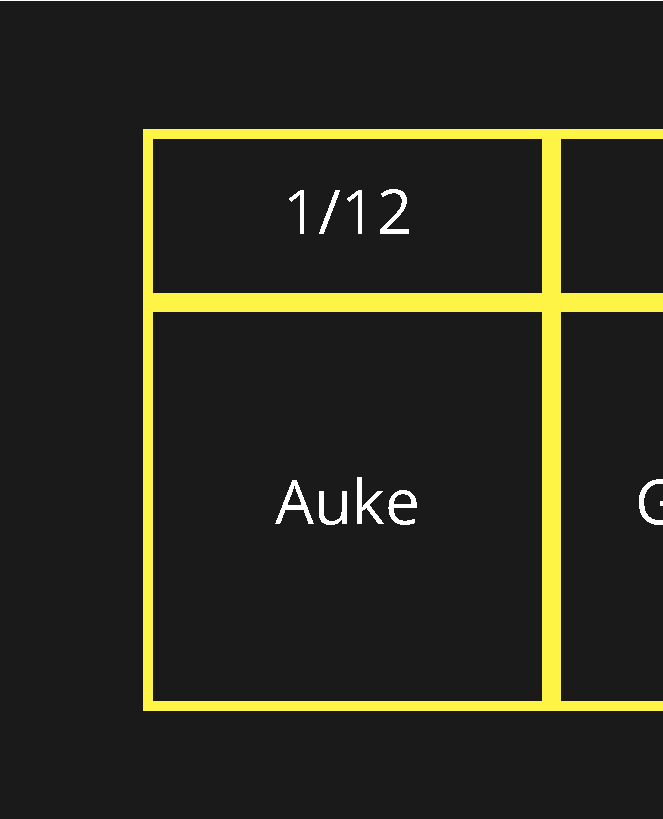
\includegraphics[scale=0.5]{binsort1.pdf}
	}
	\frame{

	}
	\frame{
		\centering
		\Huge ${O(?)}$
	}
	\frame{

	}
	\frame{
		\centering
		\Huge Gesorteerde Array: Op zoek naar Rudie
		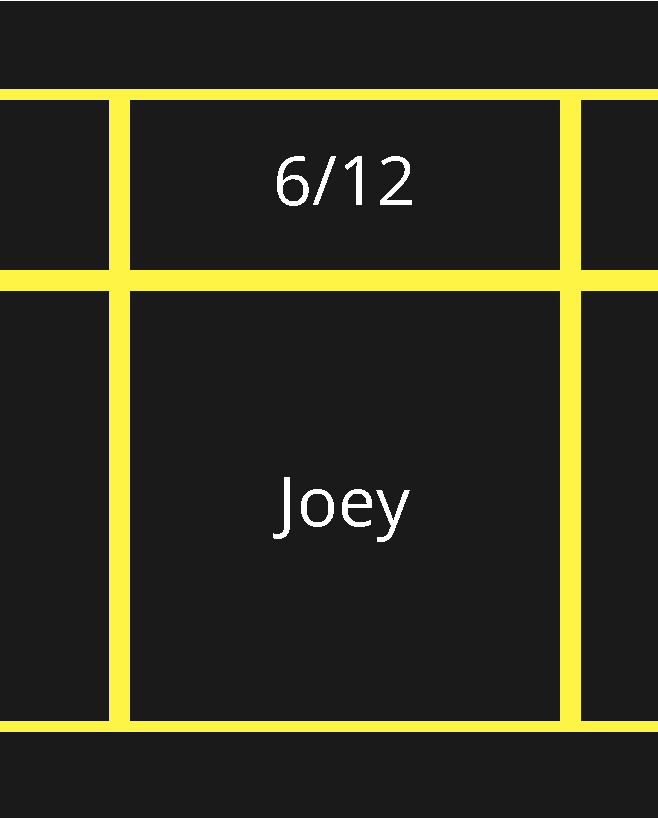
\includegraphics[scale=0.5]{binsort2.pdf}
	}
	\frame{

	}
	\frame{
		\centering
		\Huge Gesorteerde Array: Op zoek naar Rudie
		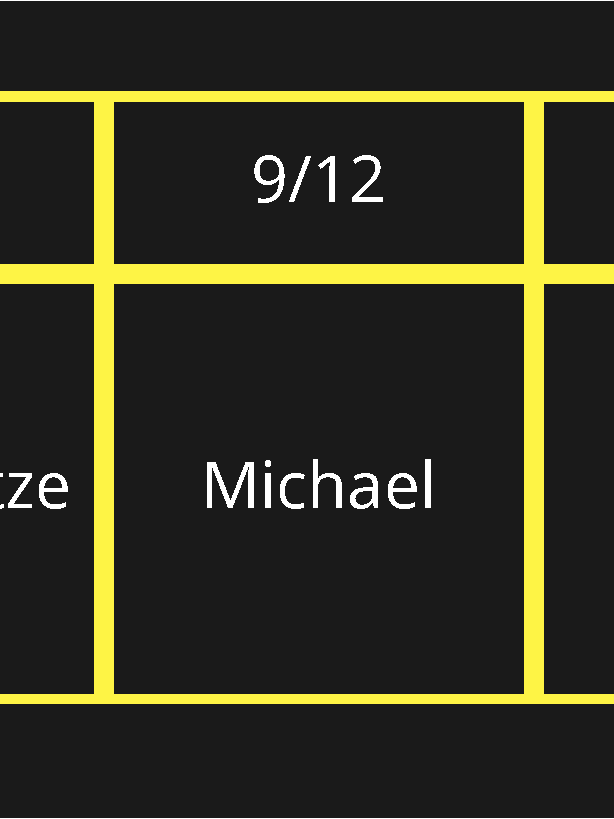
\includegraphics[scale=0.5]{binsort3.pdf}
	}
	\frame{

	}
	\frame{
		\centering
		\Huge Gesorteerde Array: Op zoek naar Rudie
		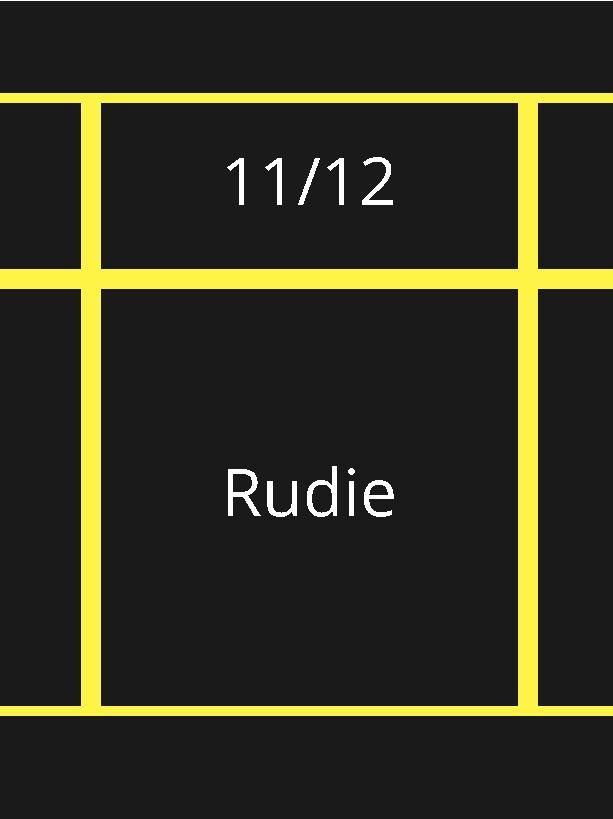
\includegraphics[scale=0.5]{binsort4.pdf}
	}
	\frame{

	}
	\frame{
		\centering
		\Huge ${O(log n)}$
	}
	\frame{

	}
	\frame{
		\centering
		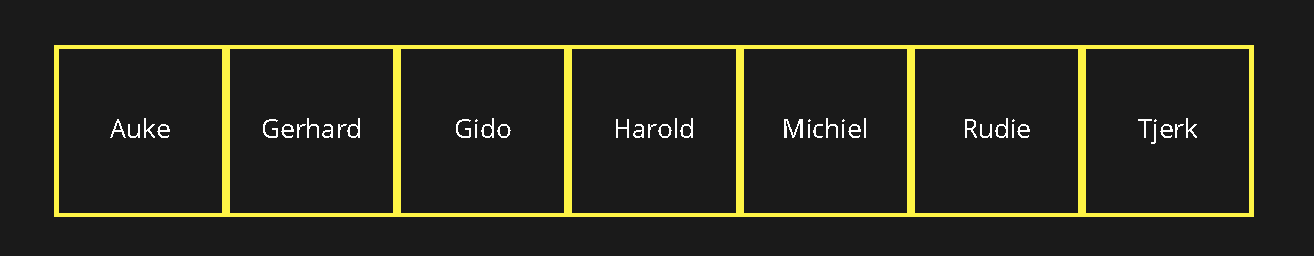
\includegraphics[scale=0.5]{array-ex}
	}	
	\frame{

	}
	\frame{
		\centering
		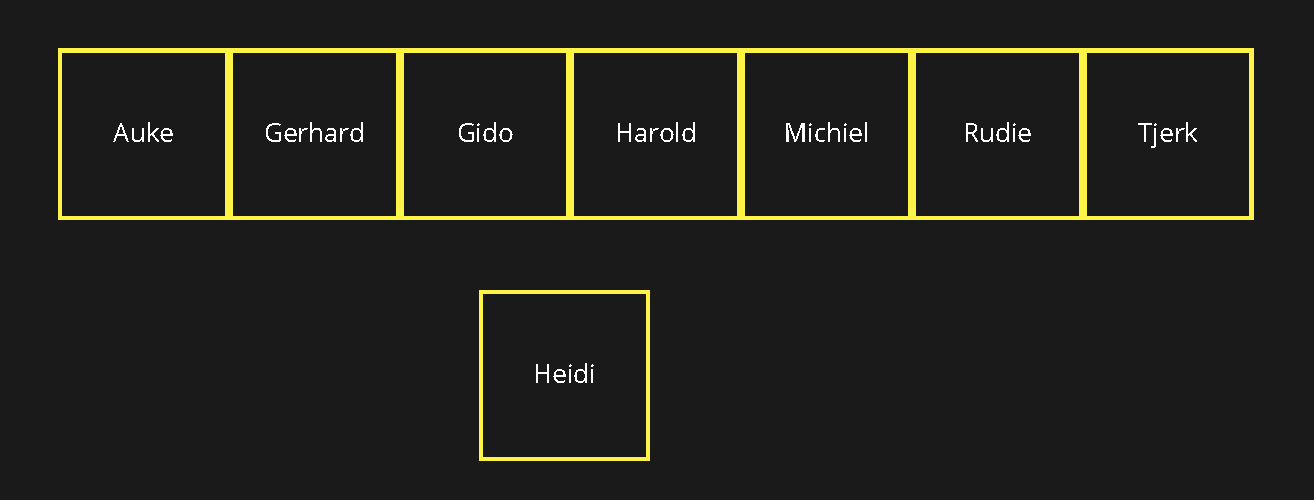
\includegraphics[scale=0.5]{array-inh}
	}	
	\frame{

	}
	\frame{
		\centering
		\Huge ${O(?)}$
	}
	\frame{

	}
	\frame{
		\centering
		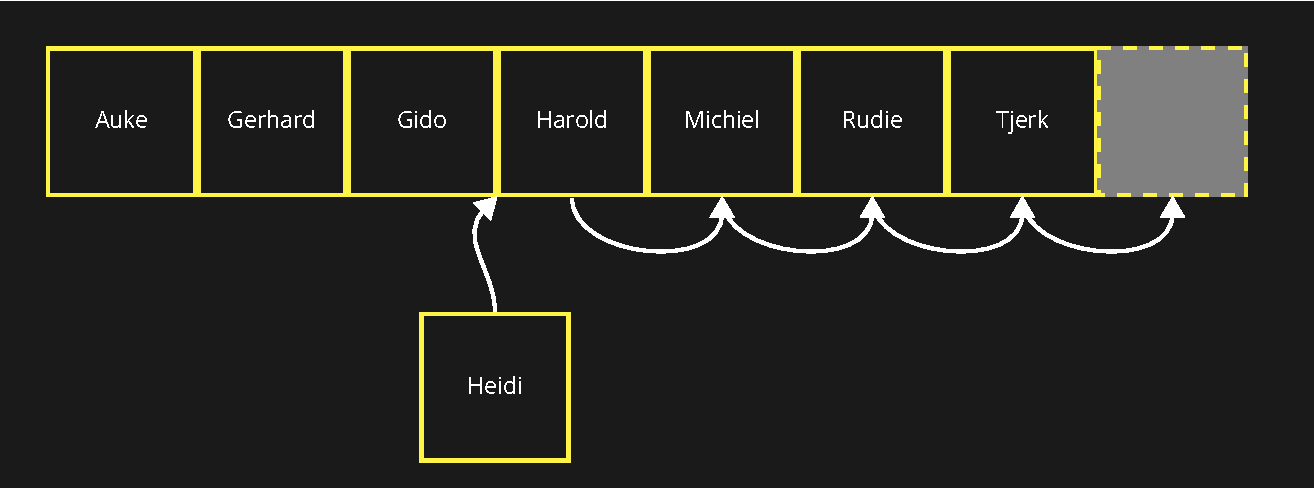
\includegraphics[scale=0.5]{array-op}
	}
	\frame{

	}
	\frame{
		\centering
		\Huge ${O(n)}$
	}
	\frame{

	}
	\frame{
		\centering
		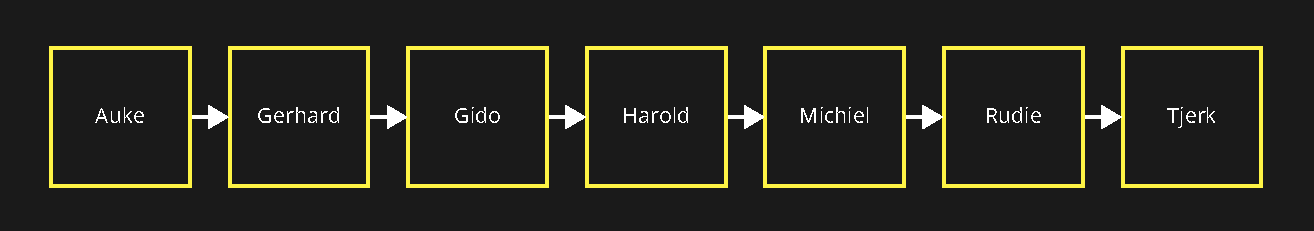
\includegraphics[scale=0.5]{linklist}
	}
	\frame{

	}
	\frame{
		\centering
		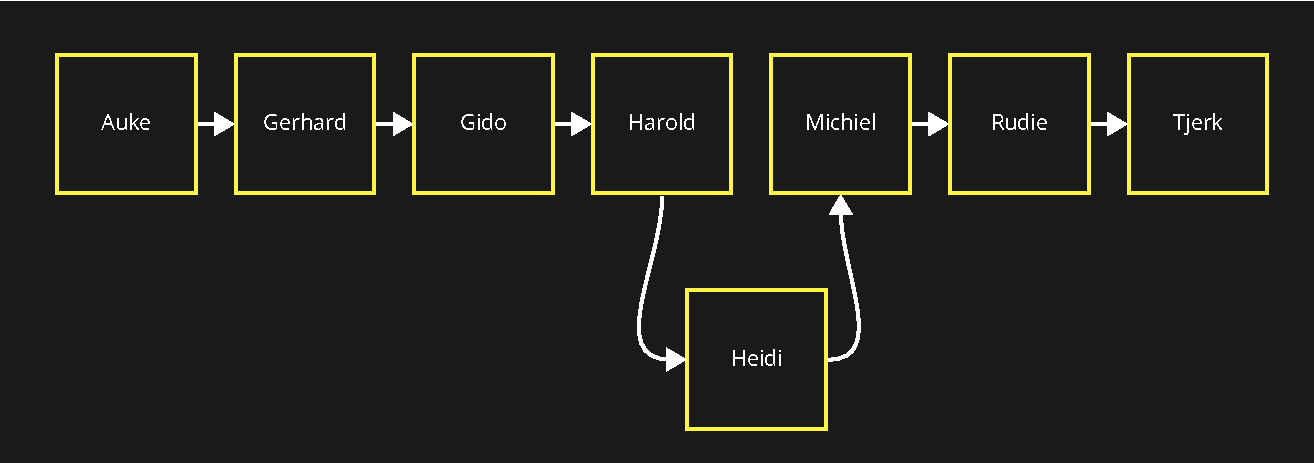
\includegraphics[scale=0.5]{linklist-insert}
	}
	\frame{

	}
	\frame{
		\centering
		\Huge ${O(1)}$
	}
	\frame{

	}
	\frame{
		\centering
		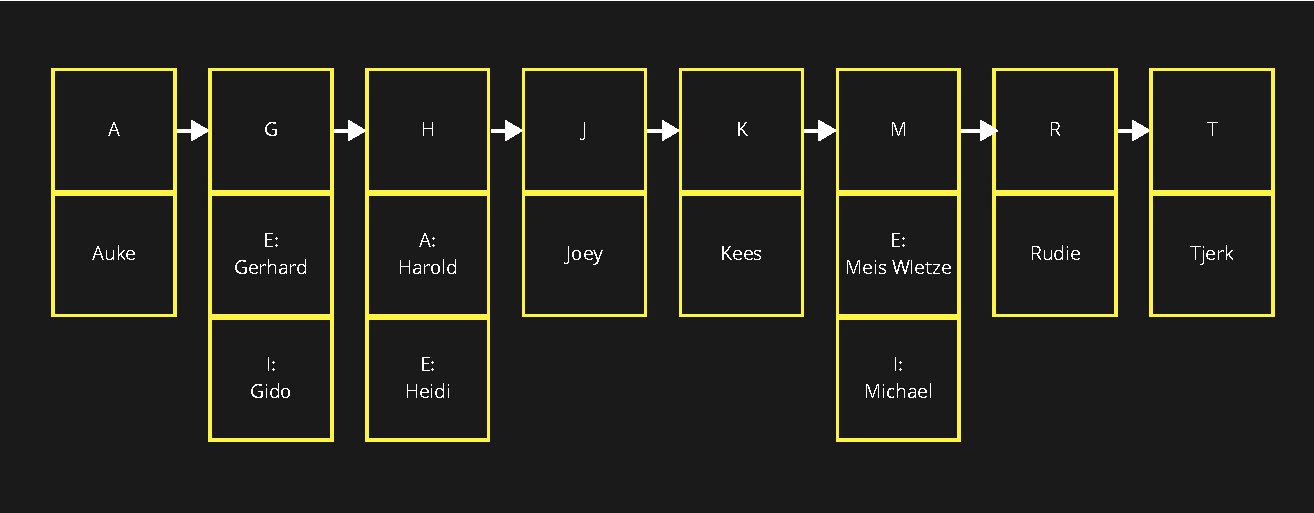
\includegraphics[scale=0.5]{tree.pdf}
	}
	\frame{

	}
\end{document}	